\section{What  \mixin Generates}\label{sec:translation}

We now show what the \mixin annotation generates. We present a formal definition for
most of the generated methods; however in our formalism we do not consider
% setters, so we do not formally define the generation of the setters.
%We do not include
casts or \Q@instanceof@, so we do not include the \Q@with@ method.
For the same reason we do not include \Q@void@ returning setters, since they are just a minor variation over the more interesting fluent setters, and they would require special handling just for the conventional \Q@void@ type.

\subsection{Translation Function}${}_{}$\\*

\noindent$[\![\mixinAnn\ \QM{interface}\ \C_0\ \QM{extends}\ \Cs \oC \methods \cC ]\!] =
\emptyset\ \QM{interface}\ \C_0\ \QM{extends}\ \Cs\ \oC
\methods\ \methods' \cC
$\\*${}_{}$\tab
where  $\valid(\C_0)$,\Q@of@$\notin\dom(\methods)$ and $\methods'=\ofMethod(\C_0) \ \otherMethod(\C_0,\methods)$.\\*

To translate an annotated interface, we add the \Q@of@ method, and then we add some other methods.
However, first of all we check if the interface is valid for annotation:

\noindent$\valid(\C_0)$  holds if $\forall \m\in\dom(\C_0),$ if $\mh\QM; = \mBody(\m, \C_0),$ one case is satisfied:
$\isField(\method)$,
$\isWith(\method, \C_0)$
or
$\isSetter(\method,\C_0)$
%$\isClone(\method, \C_0)$.

That is, we can categorize all the \emph{not implemented} methods in a pattern that we know how to implement.

%To complete our formal definition we would need to add setters and \Q@with@.
Moreover, we check that the method \Q@of@ is not already defined by the user.
In our simplified formalization we consider this to be just an error.
In our prototype we keep \Q@overloading@ into account, and so we check that an of method with the same signature of the one we would like to generate is not already present.\marco{Do we check it?}


In the following we will write $\QM{with#}\m$ to append $\m$ to \QM{with}, following the camelCase rule, so the first letter of
$\m$ must be lower-case and is turned in upper-case upon merging.
For example \QM{with#foo}=\QM{withFoo}.
Special names $\specialName(\m)$ are  \QM{with} and all the identifiers of form $\QM{with#}\m$.

\subsection{$\ofMethod$}${}_{}$\\*
We now formally define $\ofMethod$, the function that generates the method \QM{of}, that behaves like a factory. To avoid boring digressions about well known ways to find unique names, for the sake of this formalization we assume that no-args methods do not start with underscore, and we prefix method names with underscore to obtain valid  parameter names.\\*
\noindent$\begin{array}{l}
\ofMethod(\C_0) = \
 \QM{static}\ C_0\ \QM{of} \oR \C_1\ \QM_\m_1\QM,\ldots \C_n\ \QM_\m_n\cR\
\QM{\{}
\QM{return new}\ C_0 \oR\cR\ \QM{\{} \\
\tab\tab\tab\tab\tab\tab\tab C_1\ \m_1 = \QM_\m_1\QM;\ldots \C_n\ \m_n = \QM_\m_n\QM; \\
\tab\tab\tab\tab\tab\tab\tab
\C_1\ \m_1\oR\cR\ \QM{\{return }\ \m_1\QM{;\}}\ \ldots
\C_n\ \m_n\oR\cR\ \QM{\{return }\ \m_n\QM{;\}}\\
\tab\tab\tab\tab\tab\tab\tab\withMethod(\C_1,\m_1,\C_0,\es_1)\ldots\withMethod(\C_n,\m_n,\C_0,\es_n)\\
\tab\tab\tab\tab\tab\tab\tab\setterMethod(\C_1,\m_1,\C_0)\ldots\setterMethod(\C_n,\m_n,\C_0)\\
%\tab\tab\tab\tab\tab\tab\tab\cloneMethod(\C_0,\es)\\
\tab\tab\tab\tab\tab\tab\tab\withMethod(\C_0)\\
\tab\tab\tab\tab\tab\tab\QM{\};\}} \\
\end{array}$
\\*
with $\fieldsFunc(\C_0)=\C_1\ \m_1\QM{();},\ldots \C_n\ \m_n\QM{();}$,\\*
and $\es_i=\m_1\QM,\ldots\QM, \m_{i-1}\QM,\QM{_val,}\m_{i+1}\QM,\ldots\QM, \m_n$\\*
%and $\es=\m_1\QM,\ldots\QM, \m_n$\\*

The function $\fieldsFunc(\C_0)$ (formally defined later) denotes all the fields in the current interface.
For methods inside the interface with the form $\C_i\ \m_i$\QM{();}
  \begin{itemize}
   \item $\m_i$ is the field name, and have type $\C_i$.
   \item $\m_i$\QM{()} is the getter, that just return the current field value.
   \item if a method \Q@with#@$\m_i$ is required, then it is implemented by calling the \Q@of@ method using
    the current value for all the fields except for $\m_i$. Such new value is provided as parameter. This correspond to the expressions $\es_i$.
\item \QM_$\m_i$\QM($\C_i\ $\QM{ _val)} is the setter. In our prototype we use name $\m_i$, here we use the underscore to avoid modelling overloading.
%   \item similarly, for the \Q@clone@ method, \Q@of@ is called using the current value for all the fields.
   %\item To complete our generation, we need to generate setters, fluent setters and the with method.
   %\item \marco{should we just formalize setters?}
   \end{itemize}

\subsection{Other auxiliary functions}${}_{}$\\*


\noindent$\begin{array}{ll}
\withMethod:&\withMethod(\C,\m,\C_0,\es)=
\C_0\ \QM{with#}\m\oR \C\ \QM{_val}\cR\ \QM{\{}
\QM{return} \C_0\QM{.of(}\es\QM{);\}} \\
&\mbox{iff }
\mBody(\QM{with#}\m,\C_0) \mbox{ is of form }\mh\QM;\\
&\withMethod(\C,\m,\C_0,\es)=\emptyset\mbox{ otherwise}\\
\setterMethod:&\setterMethod(\C,\m,\C_0)=
\C_0\ \QM_\m\oR \C\ \QM{_val}\cR\ \QM{\{}
 \m\QM{= _val;return this;\}} \\
&\mbox{iff }
\mBody(\QM_\m,\C_0) \mbox{ is of form }\mh\QM;\\
&\setterMethod(\C,\m,\C_0)=\emptyset\mbox{ otherwise}\\
%\cloneMethod:&\cloneMethod(\C_0,\es)=
%\C_0\ \QM{clone()\{return}\ \C_0\QM{.of(}\es\QM{);\}} \\
%&\mbox{iff }
%\mBody(\QM{clone},\C_0) \mbox{ is of form }\mh\QM;\\
%&\cloneMethod(\C_0,\es)=\emptyset\mbox{ otherwise}\\
\end{array}$

\haoyuan{method name of setter?}

As you can see above, \Q@with-@ and setter methods are generated if needed.
We can discover if there is the need of generating such methods by checking if the method is unimplemented in $\C_0$. Note that we do not need to check if its header is a subtype of what we would generate, this is ensured by $\valid(\C_0)$.



\noindent$\begin{array}{ll}
\otherMethod:& \C_0\ \QM{with#}\m\oR \C\ \QM{_val}\cR\QM;\in
\otherMethod(\C_0,\methods)
\\&
 \mbox{iff }
\C\ \m\QM{();}\in \fieldsFunc(\C_0), \isWith(\mBody(\QM{with#}\m, \C_0))
\\&\mbox{ and } \QM{with#}\m\notin\dom(\methods)\\
& \C_0\ \QM_\m\oR \C\ \QM{_val}\cR\QM;\in
\otherMethod(\C_0,\methods)
\\&
 \mbox{iff }
\C\ \m\QM{();}\in \fieldsFunc(\C_0), \isSetter(\mBody(\QM_\m, \C_0))
\\&\mbox{ and } \QM_\m\notin\dom(\methods)\\
%&\C_0\ \QM{clone}\oR\cR\QM;\in
%\otherMethod(\C_0)
%\\&  \mbox{ iff }
%\isClone(\mBody(\QM{clone}, \C_0))
%\mbox{ and } \QM{clone}\notin\dom(\methods)\\
\end{array}$

Other methods that we need to generate in the interface are \Q@with-@ and setters. %\Q@clone@.
%A complete formalization would also generate the \Q@with@.
This is needed only if we need to refine the return type.
To discover if this is the case, we check if such \Q@with-@ or setter %\Q@clone@
 is required by $\C_0$, but is not already present in the methods directly declared in $\C_0$.

\noindent$\begin{array}{ll}
\fieldsFunc:&\method\in\fieldsFunc(\C_0) \mbox{ iff }
\method\in \dom(\C_0)\ \mand\ \isField(\method)
\\
\isField:&\isField(\C\ \m\oR\cR\QM;)\tab \mif\ \mnot\ \specialName(\m)\\
\isWith:&\isWith(\C'\ \QM{with#}\m \oR \C\ \x\cR\QM;, \C_0)
\tab \mif\ \C_0 <: \C', \mBody(\m, \C_0) = \C\ \m\oR\cR\QM;\\
& \mand\ \mnot\ \specialName(\m)\\
\isSetter:&\isSetter(\C'\ \QM_\m \oR \C\ \x\cR\QM;, \C_0)
\tab \mif\ \C_0 <: \C', \mBody(\m, \C_0) = \C\ \m\oR\cR\QM;\\
& \mand\ \mnot\ \specialName(\m)\\

%\isClone:&\isClone(\C\ \QM{clone}\oR\cR\QM;, \C_0)\tab \mif\ \C_0 <: \C \\
%\isImplemented:&\isImplemented(\method) \tab\mbox{iff }\method\mbox{ not of form }\mh\QM;
%\QM{default}\ \mh\mbox{\Q@\{return \_;\}@}) = \QM{true} \\
%&\isImplemented(\QM{static}\ \mh\mbox{\Q@\{return \_;\}@}) = \QM{true} \\
\end{array}$

We have not formally modelled non fluent setters and the \Q@with@ method; informally
\begin{itemize}
\item For methods inside the interface with the form \Q@void @$\m$\QM($\C\ \x$\QM{);}:
  \begin{itemize}
    \item Check if exist method $\C\ \m$\Q@();@. If not, generate error (that is, is not $\valid(\C_0)$).
    \item Generate implemented setter method inside \Q@of@:\\*
           \Q@public void @$\m$\Q@(@$\C$\Q@ _val) { @$\m$\Q@=_val;}@
    Note how there is no need to refine the return type for non fluent setters, thus we do not need to generate the method header in the interface body itself.
    \end{itemize}
\item For methods with the form $\C'\ $\QM{with(}$\C\ \x$\QM{);}:
  \begin{itemize}
    \item As for before, check that $\C'$ is a supertype of the current interface type $\C_0$.
    \item Generate implemented \Q@with@ method inside \Q@of@:\\*
           \Q@public @$\C_0\ $\Q@with(@$\C$\Q@ _val) { @\\*
           \Q@  if(_val instanceof @$\C_0$\Q@){return (@$\C_0$\Q@)_val;@\\*
           \Q@return @$\C_0$\Q@.of(@$\e_1\ldots\e_n$\Q@);}@\\*
where with $\m_1\ldots\m_n$  fields of $\C_0$,
$\e_i=$\Q@_val.@$\m_i$\Q@()@ if $\C$ has a $\m_i$\Q@()@ method; otherwise
$\e_i=\m_i$.
    \item If needed, as for \Q@with-@ and setters, generate the method header with refined return type in the interface.
 \end{itemize}

%\item For methods with the form $\C'\ \m$\QM($\C\ \x$\QM{);}:
 % \begin{itemize}
  %  \item As for before, check if exist method $\C\ \m$\Q@();@. Also, check that $\C'$ is a supertype of the current interface type $\C_0$.
   % \item Generate implemented setter method inside \Q@of@:\\*
    %       \Q@public @$\C_0\ \m$\Q@(@$\C$\Q@ _val) { @$\m$\Q@=_val; return this;}@
   % \item If needed, as for \Q@with-@ and clone, generate the method header with refined return type in the interface.
 % \end{itemize}
\end{itemize}

\marco{ insert somewhere description of  fluent setter~\cite{the lombock thread, something about fluent stuff}.
This allows for convenient and chains of setters, as we will show later \marco{insert forward reference when available}}.




\subsection{Results}
\textbf{THEOREM. }
For a given $\II_0\ldots\II_n$ interface table such that
$\forall\II\in\II_0\ldots\II_n, \II$ OK, then in the interface table
$[\![\II_0]\!]\II_1\ldots\II_n$
$\forall\II\in[\![\II_0]\!]\II_1\ldots\II_n$ either $\II$ OK or $\II$ is a subtype of $\II_0$.

To understand this theorem statement, we need to understand that there are three kind of guarantees that we can offer
\marco{should we repeat the 3 points in the email?}\\

\noindent\textbf{LEMMA 1. }
If $\II_0$ satisfies $\dom(C_0)=\dom(C_1)\cup\ldots\cup\dom(C_n)\cup\dom(\methods)$, then $[\![\II_0]\!]$ satisfies $\dom'(C_0)=\dom(C_1)\cup\ldots\cup\dom(C_n)\cup\dom(\methods)\cup\dom(\methods')$.
\begin{proof}
It suffices to prove $\dom'(C_0)=\dom(C_0)\cup\dom(\methods')$.
\begin{itemize}
\item If $m\notin\dom(\methods')$, by the definition of $\mBody$, it is obtained from $\override$. The first argument of $\override$, namely $\methods\cup\methods'(m)$, is equal to $\methods(m)$, and the second argument is not changed as well, thus the result of $\override$ is not changed during translation. Hence $m\in\dom'(C_0)$ iff $m\in\dom(C_0)$.
\item If $m\in\dom(\methods')$, we are to prove $m\in\dom'(C_0)$. So if $m$ is the $\QM{of}$ method generated by $\ofMethod$, its $\mBody$ value is well defined, by the rule $\override(\method,\none)=\method$. On the other hand, if $m$ is generated by $\otherMethod$, namely $m$ is a $\QM{with-}$ or setter method, we can also get its $\mBody$ value, since in the definition of $\otherMethod$, we can see $\isWith$ and $\isSetter$ ensure the compatible subtyping relationship. Hence $m\in\dom'(C_0)$ as well.
\end{itemize}
\end{proof}

\noindent\textbf{LEMMA 2. }
If $\II_0$ OK, then $[\![\II_0]\!]$ OK.
\begin{proof}
First assume that $\II_0$ is of form $$\mixinAnn\ \QM{interface}\ C_0\ \QM{extends}\ \overline{C}\ \oC \methods\ \cC$$
By the rule \rn{t-Invk} in Figure~\ref{ET}, we divide it into two parts.

\noindent\textbf{Part I.} For each default or static method in the domain of $[\![\II_0]\!]$, the type of the return value is compatible with the method's return type.

Since $\II_0$ OK, all the existing default and static methods are well typed in $[\![\II_0]\!]$, except for the new method \QM{of}. It suffices to prove that it still holds for $\ofMethod(C_0)$.

By the definition of $\ofMethod(C_0)$, the return value is an object $$\QM{return new}\ C_0 \oR\cR\ \QM{\{}...\ \QM{\}}$$
To prove it is of type $C_0$, we use the typing rule \rn{t-Obj}.
\begin{itemize}
\item For field typing,
\[\Gamma(\QM_ m_i)=C_i\subtype C_i\]
\item For method typing of getters,
\[\Gamma, m_i:C_i, \QM{this}:C_0, \Gamma^{\mh_i}\vdash m_i\in C_i=C^{\mh_i}\]
\item For method typing of nonempty \QM{with-} methods, by \rn{t-StaticInvk}, \haoyuan{how to do typing for the generated method itself?}
\[\Gamma, \overline{m_i:C_i}, \QM{this}:C_0, \es_i:\overline{C}_i, \Gamma^{\mh_i}\vdash C_0\QM{.of}\oR\es_i\cR\in C_0=C^{\mh_i}\]
\item For method typing of nonempty setter methods, \haoyuan{what about the \QM{with} method?}
\[\Gamma, \QM{this}:C_0, \Gamma^{\mh_i}\vdash\QM{this}\in C_0=C^{\mh_i}\]
\item To prove that $\forall i$, $\mh_i\subtype\mBody(m^{\mh_i}, C_0)$,
 \begin{itemize}
 \item For getters, \[C_i\ m_i\oR\cR\QM; \in \fieldsFunc(C_0) \Rightarrow C_i\ m_i\oR\cR\QM; \in \dom(C_0)\]
 \item For nonempty \QM{with-} methods,
  \[\begin{array}{l}
  \mBody(\QM{with#}\m_i,C_0) \mbox{ is of form }\mh\QM; \\ \valid(C_0)
  \end{array}\Rightarrow \isWith\Rightarrow C_0\subtype\mBody(m^{\mh_i}, C_0)\]
 \item For nonempty setters,
  \[\begin{array}{l}
  \mBody(\m_i,C_0) \mbox{ is of form }\mh\QM; \\ \valid(C_0)
  \end{array}\Rightarrow \isSetter\Rightarrow C_0\subtype\mBody(m^{\mh_i}, C_0)\]
 \end{itemize}
\item To prove that such a created object indeed implements all the abstract methods in $\dom(C_0)$, we simply refer to $\valid(C_0)$, since it guarantees each abstract method $\method$ to satisfy $\isField$, $\isWith$ or $\isSetter$. But that object includes all implementations for those cases, hence it is of type $C_0$ by \rn{t-Obj}.
\end{itemize}

\noindent\textbf{Part II.} Next we check that in $[\![\II_0]\!]$, $$\dom(C_0)=\dom(C_1)\cup\ldots\cup\dom(C_n)\cup\dom(\methods)\cup\dom(\methods')$$
And actually it is guaranteed by \textbf{LEMMA 1}.

\end{proof}

\begin{proof}
\textbf{(THEOREM) LEMMA 2} already proves that $[\![\II_0]\!]$ is OK. On the other hand, if some $\II$ is not a subtype of $\II_0$, the generated code in translation has no way to affect the domain of $\II$, which finishes our proof.
\end{proof}


%\subsubsection{Derived notations}
% Below shows how the functions $mtype$ and $mmodifier$ are derived from $mbody$.
%\[ \textsf{mbody}(m,C) = \textit{modifier } E \spc m(\overline{D} \spc \overline{x}) \{ \text{return } e; \} \] \[ \Rightarrow \textsf{mtype}(m,C) = \overline{D} \to E,\ \textsf{mmodifier}(m,C) = \textit{modifier}\]

%\marco{we also need to define a function that gives all the methods of an interface, something line}
%\[
%\Aux{methodsOf}_\C=\{\m|\mBody(\m,\C)=\method\}
%\]





\begin{comment}
\begin{figure}[tbp]
\centering
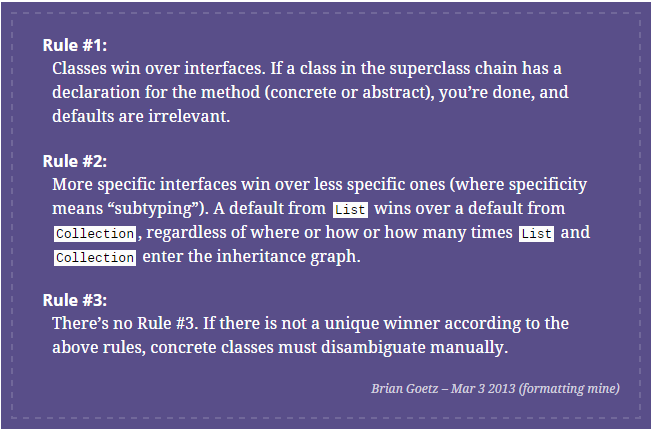
\includegraphics[width=5in]{screenshot.png}
\caption{Screenshot.}\label{screenshot_png}
\end{figure}

\haoyuan{I tried to understand the current algorithm, and did more experiments in eclipse.
Now I borrow some ideas from the current version, and give a new version of the algorithm in text. See below.

(1) I guess the function \textsf{tops} is not necessary. The first step is still
\[\textsf{mbody}(m,C_i)\in\overline{meth}\textrm{ (excluding \textbf{static} methods)}\]

(2) Assume the context is ``interface $C_0$ extends $\overline{C}$ \{$meth'$;...\}''. First handle
\[\textsf{override}(meth',\overline{meth}) \eqno{(*)}\]

(3) If $meth'\ne\none$, $(*)$ returns $meth'$ if
\[\forall meth\in\overline{meth},meth'\subtype meth\]
even if there are conflicts in $\overline{meth}$.

(4) If $meth'=\none$, we need to figure out
\[\textsf{mostSpecific}(\overline{meth})\]
and it should be the one that ``overrides'' all the others in $\overline{meth}$. It means we should not only deal with the return types of methods, but also look into the subtyping relation of interfaces. But for abstract methods, only return types are taken into consideration.
}
\end{comment}

%\text{\yanlin{shouldn't mostSpecific be: $\forall \method' \in \methods : \method \subtype
%  \method'$ ?}}

%(2) If $body_1.\textsf{returnType}=body_2.\textsf{returnType}$, \textsf{shadow} tends to return a default method. If both $body_1$ and $body_2$ are default methods, \textsf{shadow} throws an error.
%\begin{equation*}
%\begin{array}{ll}
%\textsf{shadow}(body_1, body_2)=\textsf{ERROR} & \textsf{if }body_1.\textsf{modifier}=body_2.\textsf{modifier}=\textbf{default}\\
%\textsf{shadow}(body_1, body_2)=body_1 \hspace{.1in} & \textsf{if }body_1.\textsf{modifier}=\textbf{default} \\
%\textsf{shadow}(body_1, body_2)=body_2 \hspace{.1in} & \textsf{if }body_2.\textsf{modifier}=\textbf{default} \\
%\textsf{shadow}(body_1, body_2)=body_1\textsf{ (or }body_2\textsf{)} \hspace{.1in} & \textsf{otherwise}
%\end{array}
%\end{equation*}
%
%(3) If $body_1.\textsf{returnType}<:body_2.\textsf{returnType}$, \textsf{shadow} tends to choose the one with the subtype (namely $body_1$), but only when both methods are abstract, otherwise it gives an error. The other direction $body_2.\textsf{returnType}<:body_1.\textsf{returnType}$ follows the same rule. It also gives an error if there is no subtyping relationship between two return types.
%\begin{equation*}
%\begin{array}{ll}
%\textsf{shadow}(body_1, body_2)=body_1 & \textsf{if }body_1.\textsf{modifier}=body_2.\textsf{modifier}=\emptyset\\
%& \textsf{and }body_1.\textsf{returnType}<:body_2.\textsf{returnType}\\
%\textsf{shadow}(body_1, body_2)=body_2 & \textsf{if }body_1.\textsf{modifier}=body_2.\textsf{modifier}=\emptyset\\
%& \textsf{and }body_2.\textsf{returnType}<:body_1.\textsf{returnType}\\
%\textsf{shadow}(body_1, body_2)=\textsf{ERROR} \hspace{.1in} & \textsf{otherwise}
%\end{array}
%\end{equation*}

%\subsubsection{Auxiliary function: \textsf{replace}}
%
%The \textsf{replace} function takes two same methods (with the same name and types of arguments), and gives the result of the first method overriding the second one.
%
%\begin{equation*}
%\begin{array}{ll}
%\textsf{replace}(body_1, body_2)=body_1 & \textsf{if }body_2=\emptyset\\
%\textsf{replace}(body_1, body_2)=body_2 & \textsf{if }body_1=\emptyset\\
%\textsf{replace}(body_1, body_2)=body_1 & \textsf{if }body_1.\textsf{returnType}<:body_2.\textsf{returnType}\\
%\textsf{replace}(body_1, body_2)=\textsf{ERROR} \hspace{.1in} & \textsf{otherwise}
%\end{array}
%\end{equation*}
